%\section{Relations (Not report ready (Thomas))} \todo{Need explanations and put into contest}
%
%\subsection{Physics relations}
%Relation between wavelength and frequency
%\begin{equation}
%\lambda = \frac{c}{f}
%\end{equation}
%
%Maximum Doppler frequency assuming Jakes Doppler spectrum
%\begin{equation}
%f_D=\frac{v}{\lambda}
%\end{equation}
%
%Minimum bandwidth based on Doppler frequency
%\begin{equation}
%BW = 2\cdot f_D
%\end{equation}
%
%Noise power calculation
%\begin{equation}
%w = k \cdot T \cdot BW
%\end{equation}
%
%Proportionality between variables
%\begin{equation}
%w \propto BW \propto f \cdot v
%\end{equation}
%
%\begin{where}
%\va{$\lambda$}{is the wavelength of the signal}{m}
%\va{$c$}{is the speed of light}{$\frac{\text{m}}{\text{s}}$}
%\va{$f$}{is the frequency of the signal}{Hz}
%\va{$f_D$}{is the Doppler spread}{Hz}
%\va{$v$}{is the relative velocity of the system}{$\frac{\text{m}}{\text{s}}$}
%\va{$BW$}{is the Bandwidth of the system}{Hz}
%\va{$w$}{is the noise in the system}{W}
%\va{$k$}{is Boltzmans constant}{$\frac{\text{w}\cdot\text{s}}{\text{K}}$}
%\va{$T$}{is the temperature of the system}{K}
%\end{where}
%
%
%
%\subsection{Statistical relations}
%CDF of Rayleigh fading
%\begin{equation}\label{rayleigh_CDF_std}
%p(xs < x | \theta) = 1-exp\left(-\frac{x^2}{2\cdot \theta^2}\right)
%\end{equation}
%
%
%Rewritten to SNR
%\begin{equation}\label{rayleigh_CDF}
%p(SNR < SNRs | E\left(SNR\right)) = 1-exp\left(-\frac{SNRs}{E\left(SNR\right)}\right)
%\end{equation}
%
%Closer look at the ratio from \autoref{rayleigh_CDF}
%\begin{equation}
%\frac{SNRs}{E\left(SNR\right)} = \frac{\frac{xs}{w}}{E\left(\frac{xs}{w}\right)} = \frac{xs}{E\left(xs\right)} 
%\end{equation}
%It is seen the noise does not influence the fading gain. %\todo{why does the noise not influence this?}
%
%Mean and variance of Rayleigh fading
%\begin{equation}
%\mu(x) = \theta\cdot\sqrt{\frac{\pi}{2}}
%\end{equation}
%
%\begin{equation}\label{rayleigh_var}
%var(x) = \frac{4-\pi}{2}\cdot \theta^2
%\end{equation}
%
%
%Confidence interval at $1-\alpha$ level:
%\begin{equation}\label{interval}
%\bar{x} \pm z_{\frac{\alpha}{2}} \cdot \sqrt{\frac{var(x)}{N}}
%\end{equation}
%
%Based on \autoref{interval} assuming a interval threshold, A
%\begin{equation}\label{interval2}
%N \geq \left(z_{\frac{\alpha}{2}} \cdot \frac{\sqrt{var(x)}}{A} \right)^2
%\end{equation}
%
%Using the normal approximation of the binomial proportion we  estimate the number of samples with 90\% confidence level and an interval threshold of $\pm 25\%$ or 1 dB.Based on the Equation 1.12 we have for $ \bar{x} = 10^{-5} $ :
%\begin{equation}\label{sampleEQ}
%N=(1.645)^{2} \cdot \frac{1}{(0.25)^{2}} \cdot \frac{1-\bar{x}}{\bar{x}} = 4.3 \cdot 10^{6}
%\end{equation}
%Because the above procedure is an approximation we would generate $ 10 \cdot 10^{6} $ number of samples.
%\subsection{Limitation for measurement purposes}
%
%Strict limitations
%\begin{equation}
%SNRs > 1
%\end{equation}
%
%Other limitations
%\begin{equation}
%E\left(SNR\right) \;>\, \frac{1}{raylinv(p,\theta)} 
%\end{equation}
%
%\begin{where}
%\va{$x$}{is the individual sample}{NA}
%\va{$xs$}{is a treshold value for the samples}{NA}
%\va{$\theta$}{is the mode of the distribution}{NA}
%\va{$SNRs$}{is the threshold value of the signal-to-noise ratio}{1}
%\va{$SNR$}{is the individual sample of the signal-to-noise ratio}{1}
%\va{$N$}{number of samples}{1}
%\va{$z_{\frac{\alpha}{2}}$}{is the normalize interval from a standard distribution}{NA}
%\end{where}
%
%
%
%
%\subsection{Further relations (Is this allowed?)}\todo{Have we check this?}
%
%
%From \autoref{rayleigh_CDF} and \autoref{rayleigh_CDF_std} it can be seen that
%\begin{equation}\label{thetaVsSNR}
%2\cdot\theta^2 = E\left(SNR\right)
%\end{equation}
%
%By combining \autoref{interval2} with \autoref{rayleigh_var} and \autoref{thetaVsSNR} the following relation can be obtained
%
%\begin{equation}
%N \geq \left(z_{\frac{\alpha}{2}} \cdot \frac{\sqrt{var(x)}}{A} \right)^2 = \left(\frac{z_{\frac{\alpha}{2}}}{A}\right)^2 \frac{4-\pi}{2}\cdot \theta^2 = \left(\frac{z_{\frac{\alpha}{2}}}{A}\right)^2 \cdot \frac{4-\pi}{2}\cdot \frac{E\left(SNR\right)}{2}
%\end{equation}
%
%From this relation the following proportionals can be found
%\begin{equation}
%N \propto E\left(SNR\right)\propto \frac{1}{w}
%\end{equation}
\chapter{The wireless channel}
% \chapter{Channel Dynamics} possible other headline


This chapter deals with characterization of the channel and uses the Rayleigh fading model as a theoretical baseline. The model is used to investigate the  temporal and spatial domain of a channel and how to utilize both in the measurement campaign.


\section{The Idea of Multipath}
% (basic intro / symbol introduction)
%A general way to interpret communication is by assuming two persons Alice and Bob. When Alice successfully deliver her message to Bob the communication has been a success, unfortunately Charlie likes to tease Alice and Bob by interrupting the message while its under way, making the communication a failure. The interesting part here is what happens to the message under way that determines whether it results in a success or failure. 
%In wireless communication the path travelled is what is interesting, this is especially true when more than one path is possible.
%Communication happens when a message is transmitted from a to b

In a wireless communication system the signal can reach the receiver from many different paths, this is a phenomenon called multipath propagation. It has many effects on the signal, usually on its amplitude, phase and angle of arrival.\citep{Fading} A more specific term to describe this is \textit{multipath fading}. Depending on the fading the receiver may experience constructive or destructive fading i.e. the signal might get amplified or attenuated due to the fading. Strong destructive fading is usually called deep fades and can lead to outages of the communication system for short periods of time. 

Fading can be separated in  small scale and large scale fading \citep{FlatSelective}: 

\begin{tabular}{lp{13.1cm}}
\textbf{Large scale} & is often called the path loss and is dependent on the distance between receiver and transmitter along with the terrain and obstacles in the area. \\ 
\textbf{Small scale} & is a more stochastic measure, which is dependent on small changes in position of either the receiver, transmitter or obstacles. These changes might be very small down to mm or cm compared to the overall distance which might be km, however the effects can be very severe. Small scale fading is further split up into frequency flat and frequency selective fading:
\end{tabular}
\begin{tabular}{p{0.3cm}lp{11.7cm}}
&\textit{Flat Fading} & All the frequencies experience the same changes in amplitude and phase over a period of time, this is seen as a change in SNR.\\
&\textit{Selective Fading} & Different frequencies across the channel experience different changes in amplitude and phase. 
\end{tabular}



%\begin{Symbol List}
%\vaSB{$c(t)$}{Rayleigh continues-time channel impulse response}{NA}
%\vaSB{$t$}{Time}{s}
%\vaSB{$a$}{Amplitude}{NA}
%\vaSB{$\Psi$}{Phase}{NA}
%\vaSB{$\tau$}{time delay or time shift}{s}
%\vaSB{$\delta$}{Dirac delta}{1}
%\vaSB{$N$}{number of samples}{Na}
%\vaSB{$\psi$}{combination argument of $\Psi$ and $\tau$}{NA}
%\vaSB{$i$}{imaginary number}{NA}
%\vaSB{$C(t)$}{Rayleigh impulse response process}{NA}
%\vaSB{$\left | \cdot \right |$}{absolute value of $|\cdot|$}{NA}
%
%\vaSB{$\mathbb{E}{[\cdot]}$}{Expectation of $[\cdot]$}{NA}
%\vaSB{$f$}{Frequency}{1/s Hz}
%\vaSB{$h(t)$}{physical process as a function of t}{NA}
%\vaSB{$H(t)$}{physical process as a function of f}{NA}
%\vaSB{$\mathcal{F}$}{Fourier transform}{NA}
%\vaSB{$D\mathcal{F}$}{Double Fourier transform}{NA}
%\vaSB{$\Delta d$}{Space, displacement}{m,$m^2$}
%\vaSB{$f_d$}{Spatial frequency, Doppler}{1/m}
%\vaSB{$R$}{Autocorrelation}{NA}
%\vaSB{$S$}{Power Spectral density PSD}{NA}
%\vaSB{$\lambda$}{wavelength}{m}
%
%\vaSB{$BW$}{Bandwidth}{Hz}
%\vaSB{$B_c$}{Coherence Bandwidth}{Hz}
%
%\vaSB{$\sigma_{\tau}$}{RMS delay spread}{NA}
%\vaSB{$f_c$}{Carrier frequency}{Hz}
%
%\vaSB{$\delta$}{Area}{$m^2$}
%\vaSB{$A_{div}$}{Antenna array diversity}{NA}
%%%\vaSB{$$}{}{}
%\end{Symbol List}

\subsection{Diversity}
% (effects?)
Diversity is used to combat fading in a wireless system. By using clever techniques you can effectively deliver several copies of a signal to the receiver. The probability that all copies experience deep fades is smaller than having only one copy experience deep fade \citep[p. 4-6]{diversityFuture}. The overall goal is to provide a gain in signal quality by having several signals that independently fade from each other with as little cost as possible in power consumption, bit rate, system complexity or other resources. There are several ways to achieve diversity in a wireless system. \\
Temporal diversity: By retransmitting the same information you get some diversity gain on the cost of decreased bit/rate. Usually a forward error correction code is added instead of just re transmitting the signals several times. \\
Antenna diversity / Spatial diversity:
By having several antennas at either or both the receiver and transmitter, antenna diversity is achieved. Separating the antennas around half a wavelength the signals get uncorrelated and become independently fading signals, that can be combined together into one achieving a processing gain \citep{diversityAntenna}. Antenna diversity comes at the cost of a more complex system or increased power consumption.


	
\section{Rayleigh Fading} \todo{sources for the text}
% (confidence level vs number of samples)

%\section{Statistics}
%\subsection{Confidence Interval}
%\subsection{Distributions?}


Rayleigh fading is a propagation model that is used to describe situations where there are no line of sight connections and the signal may vary randomly due to scatterings. Usually this situation fits on an urban environment scenario with many buildings and obstacles. In \autoref{eq:reyl_impulse_response} the impulse response of a Rayleigh fading channel can be seen \citep{MeasurementComplexRay}.
\begin{equation}\label{eq:reyl_impulse_response}
c(t;\tau) = \sum_{n =0}^{N} a_n(t)e^{j\Phi_n(t)} \delta (t-\tau_n(t))
\end{equation}

\begin{where}
\va{$c(t;\tau)$}{is the impulse response of a fading channel}{1}
\va{$t$}{is absolute time}{s}
\va{$\tau$}{is delay from t}{s}
\va{$N$}{is the number of reflective paths}{1}
\va{$a_n$}{is the attenuation of the path}{1}
\va{$\Phi_n$}{is the phase change of the path}{rad}
\end{where}

%In narrowband transmissions  the multipath propagation experiences rapid fading in the signal envelope and in the received spectrum the Doppler spread is clearly visible.  

%To do a measurement of a wireless channel need to have sufficient number of samples to have a certain error margin and confidence interval. To simplify one can only look at  the noise free case to see what different properties we can change to reduce the amount of samples we need. 
It should be mentioned that $t=0$ is assumed to be the time the first signal is received. If $N \rightarrow \infty$ the fading channels for a narrow band system can be expressed as \autoref{eq:inf_reyl_impulse_response} \citep{MeasurementComplexRay}. 

\begin{equation}\label{eq:inf_reyl_impulse_response}
C(t) = \left [ \sum_{n =1}^{N} a_n(t)\cdot cos(\psi_n (t))\right ] + j\left [\sum_{n =1}^{N} a_n(t)\cdot sin(\psi_n (t))  \right ]
\end{equation}
\begin{where}
\va{$C(t)$}{is the impulse response of a Rayleigh fading channel}{1}
\va{$\psi_n(t)$}{is due to $\Phi_n(t)$ and $\tau_n(t)$ and is induced by the Doppler shift}{rad}
\end{where}

If we assume that the random variables is not dependent on time, the impulse response process $C(t)$ will be \gls{WSS}. Given the central limit theorem that states:
"\textit{...the distribution of the sum (or average) of a large number of independent, identically distributed variables will be approximately normal, regardless of the underlying distribution}" \citep{CentralLimit}.  
Assuming that the phase is uniformly distributed between [$-\pi,\pi$], both the real and imaginary parts can be treated as Gaussian processes with a mean of zero and equal variances. This is the fundamental underlying assumption of a Rayleigh fading channel and $ \left | C(t) \right | $ becomes a Rayleigh random variable \citep[p. 589]{Wireless_CommunicationsBook}. The squared-envelope $ \left | C(t) \right |^2 $ is the instantaneously fading gain at time t. A measurement is typically made of $ \left | C(t) \right |^2 $ from which $ \mathop{\mathbb{E}}\left | C(t) \right |^2 $ is estimated to find the average power of the fading gain. To obtain some measurement samples of $ \left | C(t) \right |^2 $ one can transmit testing signals witch are identically disturbed and estimate the mean \citep{MeasurementComplexRay}.



%When measuring narrowband channels in a indoor environment the usual deep fades seen are not lower then -20dB off the mean value of the signal, due to the fact that only a small amount of samples are used (<100) the deep fades that the Rayleigh model predicts ($10^{-5}$) has such a low chance of happening that number of samples needs to be unreasonable high in a normal measuring case.

\section{Doppler shift}
Doppler shift is when the relative velocity of of the receiver compared to the transmitter causes a frequency shift for the signal of each path. The \gls{BW} of a system must be larger then the maximum Doppler shift to work. The maximum Doppler shift is related to the velocity by \citep[p. 229]{Wireless_CommunicationsBook}:
\begin{equation}\label{eq:Doppler}
f_d = \frac{2}{\lambda} \cdot v
\end{equation}
\begin{where}
\va{$f_d$}{is the maximum Doppler shift}{Hz}
\va{$\lambda$}{is the wavelenght}{m}
\va{$v$}{is the relative velocity of the receiver compared to the transmitter}{$\frac{m}{s}$}
\end{where}

%If we assume the system is moving slowly at $5m/s$ and we use an open $2.4Ghz$ \todo{is these the values we expect} frequency we can see that the Doppler spread is 80Hz. This means our bandwidth can't be lower than 80 Hz. We know that the dynamic range of system is dependant on the IF bandwidth, and that we should use as low BW as possible \todo{source}. A 80 Hz bandwidth is very narrow and will give us little frequency dependant fading and we can assume frequency flat fading \todo{source}. Given this definition of Doppler spread we can assume that this should not be a problem since our measurements BW must be higher to get enough samples \todo{source}.

\section{Wireless channel characteristics}

%To accomplish a measurement with some degree of accuracy (confidence interval) we must understand the statistics and the parts that affect it. One thing that is clear though is that many uncorrelated samples are needed. We will assume that we need $10^7$ uncorrelated samples to get some degree of accuracy for $10^{-6}$ probability. Now how do we get $10^7$ uncorrelated samples?
%There are several physical limitations that need to be balanced  in order to prove the claims of the Rayleigh fading model with a predefined confidence interval and to obtain a large amount of uncorrelated samples.
%\todo {Remove this first part?}

Wireless multipath fading channels are characterized in two domains, namely the temporal and spatial domains \citep[p. 40-42]{stochasticWirelessChan}. To achieve the desired amount of samples found in \autoref{sec:statistics}, utilization of both domains are necessary. The reason for this is the limited timeframe and available locations for the project.
%These domains are connected\todo{how} and must be balanced to make the measurement campaign plausible. We have time constraints; as in we can't take measurements for several years. Space constraints; as we have a limited amount of space to measure.
% Frequency constraints; to get high enough dynamic range to see very severe fading (-60dB) we are limited on bandwidth.

%A typical physical process can be described further by splitting up the two domains into two different representations.In the time domain with some values of quantity $h$ as a function of time $t \ [s]$, so $h(t), -\infty < t < \infty$. The second representation is a function of frequency $f \ [\frac{1}{s}]$ by a complex number $H$,which gives amplitude and phase as a function of the frequency, $f$ that is $H(f) -\infty < f < \infty$. These can be though of as two different representations that are connected by Fourier transforms.

The domains can further be split up into two different representations. In the temporal domain the channel can be a function of time or a function of frequency. These are two different representations that is connected by the Fourier transform as seen in \autoref{eq:temporal1} \citep[p. 43]{Wireless_CommunicationsBook}.

\begin{equation}\label{eq:temporal1}
%H(f)=\int_{- \infty}^{\infty}h(t)e^{-2\pi ift} dt \quad \Leftrightarrow \quad
%h(t)=\int_{- \infty}^{\infty}H(f)e^{2\pi ift} df
G_t(f) = \mathcal{F}(g_t(t))
\end{equation}
\begin{where}
\va{$G_t(f)$}{is the frequency representation of the channels temporal domain}{1}
\va{$g_t(t)$}{is the time representation of the channels temporal domain}{1}
\end{where}

%In the spatial domain the representations are with some values of quantity $g$ as a function of space $\Delta d \ [m]$, so $g(\Delta d), -\infty < \Delta d < \infty$. The second representation is a function of the spatial frequency $f_d \ [\frac{1}{m}]$ by a complex number $G$,which gives amplitude and phase as a function of the spatial frequency(Doppler), $f_d$ that is $G(f_d) -\infty < f_d < \infty$.
%These can be though of as two different representations that are connected by Fourier transforms.

The spatial domain can equally be a function of space or spatial frequency, which is also related by the Fourier transform as seen in \autoref{eq:spatial1} \citep[p. 43]{Wireless_CommunicationsBook}.

\begin{equation}\label{eq:spatial1}
%G(f_d)=\int_{- \infty}^{\infty}g(\Delta d)e^{-2\pi ift} d\Delta d \quad \Leftrightarrow \quad
%g(\Delta d)=\int_{- \infty}^{\infty}G(f_d)e^{2\pi ift} df_d
G_s(f_d) = \mathcal{F}(g_s(d))
\end{equation}
\begin{where}
\va{$G_s(f_d)$}{is the spatial frequency representation of the channels spatial domain}{1}
\va{$g_s(d)$}{is the space representation of the channels spatial domain}{1}
\end{where}


%If the units of $\Delta d$ is meters,then $f_d$ is in cycles per meter. The $\Leftrightarrow$ represents the Fourier transform. 
The spatial domain is 3 dimensional given as $d = (x,y,z)$, in the analysis this can however be limited to 1 or 2 dimensions for simplicity \citep{FTandCORR}.

%Here is the time delay space relationship Fourier transform pair. This gives us the deterministic or instant transfer functions:
These domains and their representations can be combined in four different ways which is related by the Fourier transform as seen in \autoref{eq:channel_rep1} \citep[ch. 6.3]{The_Mobile_Radio_Propagation_Channelbook}.

\begin{center}
$h(d,t)$\\
\scalebox{0.75}{
${\mathcal{F}\downarrow \uparrow \mathcal{F}^{-1}}$}\\
$S(f_d,t)$ $\quad \quad$ $T( d,f)$\\
\scalebox{0.75}{
${\mathcal{F} \downarrow \uparrow \mathcal{F}^{-1}}$}\\
\vspace{-1.9em}
\begin{equation}\label{eq:channel_rep1}
H(f_d,f)
\end{equation}
\end{center}
\begin{where}
\va{$h(d,t)$}{is the space variant impulse response function}{1}
\va{$S(f_d,t)$}{is the output Doppler scattering function}{1}
\va{$T(d,f)$}{is the Doppler-delay scattering function}{1}
\va{$H(f_d,f)$}{is the space variant transfer function}{1}
\end{where}
%$\Delta d$ is separation in space, $\tau$ is time delay ,$f$ is frequency, $f_d$ is the Doppler.



\section{Wide sense stationary uncorrelated scattering}

Since the channel behaviour is hard to predict, the normal method is to use statistical models to describe a channel in terms of probabilities. So the channel impulse response is considered a random process. The \gls{ACF} of the channel is used to characterize changes in time and space.

In a \gls{WSSUS} channel model the correlation function is time invariant and that the different scatters and their delays are uncorrelated. This means that the ACF of the channel only need one parameter per domain, because only the change in position and time affects the channel. WSSUS model gives a realistic way to describe short term fading of the channel \citep[ch. 6.5-6.6]{The_Mobile_Radio_Propagation_Channelbook}.

This means that the general ACF can be simplified as seen in \autoref{eq:acf1}.
\begin{equation}\label{eq:acf1}
R_{h}(d,d+\Delta d,t,t+\tau) = R_{h}(\Delta d,\tau) 
\end{equation}
\begin{where}
\va{$R_{h}$}{is the \gls{ACF} of $h(d,t)$}{1}
\va{$\Delta d$}{is a change in position}{m}
\va{$\tau$}{is a time delay}{s}
\end{where}

%The $|R(\tau)| = \mathop{\mathbb{E}}(h(t))^2)$ \todo{check source does not seem true}, which is the average power of $h(t)$. Under the same assumption of WSS the ACF of $g_s(d)$ in the spatial domain is also only dependent on the spatial offset, $\Delta d$. 
The relation between joint autocorrelations are found using Fourier transform \citep[ch. 6.5-6.6]{The_Mobile_Radio_Propagation_Channelbook}:
%\begin{center}
%$R_h(\Delta d_1,\Delta d_1,\tau_1,\tau_2)$\\
%\scalebox{0.5}{
%${D\mathcal{F}\downarrow \uparrow D\mathcal{F}^{-1}}$}\\
%$R_S(f_{d1},f_{d2},\tau_1,\tau_2)$ $\quad \quad$ $R_T(\Delta d_1,\Delta d_2,f_1,f_2)$\\
%\scalebox{0.5}{
%${D\mathcal{F} \downarrow \uparrow D\mathcal{F}^{-1}}$}\\
%\vspace{-1.9em}
%\begin{equation}
%R_H(f_{d1},f_{d2},f_1,f_2)
%\label{AutocorrDouble}
%\end{equation}
%\end{center}

\begin{center}
$R_h(\Delta d,\tau)$\\
\scalebox{0.75}{
${\mathcal{F}\downarrow \uparrow \mathcal{F}^{-1}}$}\\
$R_S(f_{d},\tau)$ $\quad \quad$ $R_T(\Delta d,\Delta f)$\\
\scalebox{0.75}{
${\mathcal{F} \downarrow \uparrow \mathcal{F}^{-1}}$}\\
\vspace{-1.9em}
\begin{equation}
R_H(f_{d},\Delta f)
\label{AutocorrDouble}
\end{equation}
\end{center}

\begin{where}
\va{$R_h(\Delta d,\tau)$}{is the ACF of the space variant impulse response function}{1}
\va{$R_S(f_{d},\tau)$}{is the ACF of the output Doppler scattering function}{1}
\va{$R_T(\Delta d,\Delta f)$}{is the ACF of the Doppler-delay scattering function}{1}
\va{$R_H(f_{d},\Delta f)$}{is the ACF of the space variant transfer function}{1}
\end{where}



 %The \gls{PSD} $S_H(f_d, \Delta f)$ measure the instant spectral power in a random channel. The PSD is non negative and symmetrical. 
%The autocorrelation is related to the \gls{PSD} by another Fourier transform. One can transform from PSD to autocorrelation by a inverse Fourier transform for the temporal and spatial domain. 
In the measurement campaign knowledge about the correlation related to the change in position and shift in frequency is relevant as these parameters are typically the ones to manipulate. With out the actual measurements it is however often easier to get information of the correlation to the time delay and the Doppler spectrum, and a conversion between the parameters has to be performed using the relation described in \autoref{AutocorrDouble}.
To help in the analysis it is assumed the two domains are independent and therefore analysis of the \gls{SCF} and \gls{FCF} can be done separately.


%\begin{equation}
%S_H(f_d, \Delta f) = \mathcal{F}(R_H(f_{d},\Delta f))
%\end{equation}


%\begin{equation}
%S(\Delta f) = \mathcal{F}(R(t))
%\end{equation}
%\begin{equation*}
%S [cylces \ per \ second] \Leftrightarrow R [second]
%\end{equation*}
%
%\begin{equation}
%S(f_d) = \mathcal{F}(R(\Delta d ))
%\end{equation}
%\begin{equation*}
%S [cylces \ per \ meter] \Leftrightarrow R [meter]
%\end{equation*}

%where S is the PSD and R is the autocorrelation. $\mathcal{F}$ represents the Fourier transform. 

%Doppler, delay and wave number spectra are defined and we can use Fourier transform to find the Autocorrelation. In reality we want to look at relationships between factors that affect a random channel, with the joint autocorrelation functions and joint PSDs\citep{SpaceWirelessChan}.


%\begin{equation}
%D\mathcal{F} ( h(t,f,L) ) =
%D\mathcal{F}^{-1} ( H(f_d,\tau,\Delta d) )
%\end{equation}
%$D\mathcal{F}$ is the double Fourier transform where $t$ is absolute time,$f$ is frequency and $L$ position in space(1 dimension).
%Where $f_d$ is the Doppler, $\tau$ is the time shift and $\Delta d$ is the separation in space (wave number).




%\begin{equation}
%\huge{\ h(\Delta d,\tau)}  \\ \small {\mathcal{F} \downarrow \uparrow \mathcal{F^{-1}}} \\ \huge {S(f_d,\tau) \quad\quad\quad T(\Delta d,f)} \\
%\small {\mathcal{F} \downarrow \uparrow \mathcal{F^{-1}}} \\
%\huge {\ H(f_d,f)}
%\end{equation}


%\begin{equation}
%\mathcal{F} ( h(t,\Delta d) ) =
% S(f_d,\tau) )
%\end{equation}
%where $f_d$ is Doppler and $\Delta d$ is separation in space.


%\section{Coherence functions}
\subsection{\Gls{SCF}}
As seen from \autoref{AutocorrDouble}, the SCF can be found by taking the Fourier transform of the Doppler spectrum. 

\begin{equation}
R_{h}(\Delta d) = \mathcal{F}(R_{S}(f_d))
\end{equation}

By assuming a frequency of 4 GHz and using \autoref{eq:Doppler}

The measurement points needs to be spaced $\Delta d = \frac{\lambda}{2}$ to let the measurement points have independent fading. This is assuming a uniformly distributed angle of arrival given:
\begin{equation}
R_g[\Delta d] = J_0(2\pi \frac{\Delta d}{\lambda})
\end{equation}
Where $R_g$ is the autocorrelation function in space $\Delta d$ is the difference in distance. $J_0$ is the Bessel function with order 0.
We want the correlation to be close 0 so the fade is uncorrelated. The first zero of the $J_0$ function is at 2.4048 \citep[p.335]{Jakes_microwave}.

\begin{figure}[H]
\centering
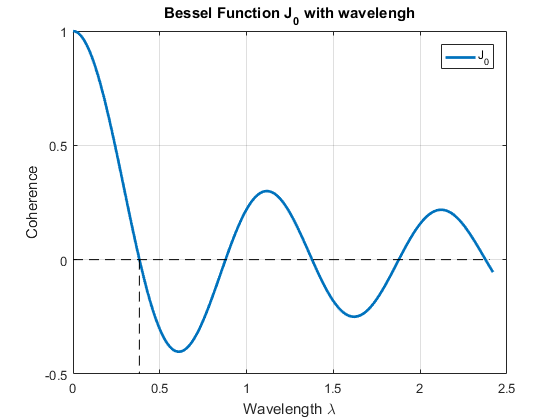
\includegraphics[width=0.75\textwidth]{figures/Bessel_wavlength.png}
\caption{The coherence function scaled by wavelength.}
\label{bessel_wave}
\end{figure}


\begin{equation}
\frac{2\pi \Delta d}{\lambda} = 2.4048 \Leftrightarrow \Delta d = 0.38 \lambda \approx \frac{\lambda}{2}
\end{equation}

If the frequency is low then it might be difficult to have a sufficient amount of independent fading measuring points. \citep[p.11]{UWMeasurement} Too get uncorrelated  parallel measurement a antenna array with $\frac{\lambda}{2}$ separated antennas can be used for multi probe measurements. A antenna array will multiply the number of samples measured at each time interval of the reviver and transmitter. So a $5\cdot 5$ antenna array would gives us $5^2 = 25$ uncorrelated channels each measurement.

%The other part of the Fourier transfer pairs is the time frequency relationship joint PSD and Autocorrelation:
%\begin{equation}
%\mathcal{F} ( h(t,f) ) =
% S(f_d,\tau) )
%\end{equation}
%Where $t$ is time and $f$ is frequency. The autocorrelation function $S{f_d,\tau}$ is defined by the Doppler $f_d$ and the delay $\tau$



The sample size can be further increase by using uncorrelated samples in the frequency domain. 
For samples to be uncorrelated a frequency separation $\Delta f$  is needed. This has to be as big as the coherence BW. $B_{c}$. $B_{c}$ is statistical and measurement dependant on the relationship between different frequencies over the channel that has a strong correlation.The Fourier transform of the PDP gives the Frequency correlation function that is used for determining the coherence bandwidth of the channel. This is dependant on the actual environment in which measurements are conducted. A exact value has to be determined from  an actual measurement of the channel, but there are approximations\citep{RayFadeHandbook}. The RMS delay spread $\sigma_{\tau}$ is given by:
\begin{equation}
\sigma_{\tau} = \sqrt{\bar{\tau} - {(\bar{\tau}^{2})}}
\end{equation}
Where $\bar{\tau}$ is the mean excess delay $(\bar{\tau}^{2})$ is 
the second central moment of $H(\tau)$. With the RMS delay spread we can find $B_c$ by approximation:
\begin{equation}
B_C \geq \frac{1}{2\pi \cdot \sigma_{\tau}}
\label{CohBW}
\end{equation}
This will gives us a $B_c$ approximation that has a coherence under 0.5. The coherence function will go towards 0 as $B_c  \rightarrow \infty $
\citep{CohBW}
If we look at a example from lecture at AAU we got a $B_c$ of 10 Mhz in a multipath lab environment.
\todo{might be somthing wrong with the matlab script, because the FCF shows more BW} With a delay profile of around 20ns. So in a small environment with small delay profile a larger $\Delta f$ is needed to have samples uncorrelated.
\citep[Chapter 18.5]{ComHandbook}

\subsection{How to measure uncorrelated samples}
\label{howtomeasureUS}
\todo {rewrite in more general term and then use example values or make table}
To measure the required samples from \autoref{sampleEQ} ($\approx 4.04\cdot10^6$) uncorrelated samples requires a elaborate test setup. The limitation is in how much space and time the measurement is going to require. The example scenario  will have a $f_c$ of 3Ghz, BW of 100MHz, a $5x5$ antenna array, a office building with a delay spread of 100ns and a room size that is $10m \cdot 10m$.
If we assume we have a multipath delay spread of 100ns. Given \autoref{CohBW} the $B_C$ is 1.6MHz. Since the $B_C$ is only a approximation with some coherence, the $B_C$ should be increased to approximate 3 Mhz to get less correlated samples. This will give round 30 uncorrelated samples in frequency with a BW of 100MHz.
The $f_c$ of 3Ghz gives a $\lambda$ of 0.1m or 10cm. The array antennas has each antenna spaced half a $\lambda$ which would give a total antenna length of 0.25m. If the antenna array is moved in one dimension,every step needs to be spaced $0.25+\frac{\lambda}{2}$ apart. Given the 10m size of the room 30 samples is possible in 1 dimension. If the measurements is done in 2 dimensions ($10m\cdot 10m$) a total area of:

\begin{equation}
N = \underbrace{A_{div}}_\text{$N_a$} \cdot \underbrace{\frac{BW}{B_c \cdot 2}}_\text{$N_f$} \cdot \underbrace{\frac{\Delta}{(\frac{\lambda}{2})^2}}_\text{$N_d$}
\label{howtosample}
\end{equation} 
 
Where $N$ is number of samples(in antenna diversity,frequency and space), $A_{div}$ is the antenna diversity, $\Delta$ is the area, $B_c$ is the coherence BW and $\lambda$ is the wavelength.
\autoref{howtosample} can be used to found the area required given number of samples $N$ needed.
\begin{equation}
\Delta  = \frac{N\cdot (\frac{\lambda}{2})^2}{A_{div}\cdot \frac{BW}{B_c \cdot 2}}
\label{howtosqaure}
\end{equation}
If we assume a $10m \cdot 10m$ this gives us: 
\begin{equation}
\frac{10m}{\frac{\lambda}{2}} \cdot \frac{10m}{\frac{\lambda}{2}}  = 40000 samples
\end{equation}
The total amount of spatial, frequency and antenna array uncorrelated samples is:
\begin{equation}
30 \cdot 25 \cdot 40000 = 3 \cdot 10^7 samples
\end{equation}
which is way more then we need.
Actually moving the reviver $2 \cdot 10^6$ times takes way to long to actually do, but this example calculation is just to show that it is possible to obtain $10^7$ samples.If the area of the measurement is not big enough to take all the measurements different rooms could be used. To do this you need to normalize for the mean gain the system sees. 

A other problem with a taking $10^7$ samples is that the channel may be changing because of frequency shift or movement. This will make the samples uncorrelated, but you are in danger of measuring a completely different channel. Here comes the non-stationary principle into play. A argument could be made that the $10^{-6}$ fading is so dependant on the environment that a measurement would only be valid for this exact room or situation you are measuring.

\subsection{Time required to do measurements}
When trying to obtain a high number of samples, time becomes a very limiting factor. For this reason a estimation of total measurement time or a time budget is helpful. If one sample takes 1 second to measure and the required samples size is $10^7$, the total measuring time would be 116 days of continues measurements. This of course is not practical to do. So it's obvious that a automatic systems that takes several samples in parallel is needed. The time budget uses the values from  \autoref{howtomeasureUS} and assumes the samples are measured continuously in one dimension with a velocity of $1m/s$. 
The antenna array is spaced in a different dimension so samples don't overlap. The time it would take to do a $100MHz$ sweep is dependant on the $IF_{BW}$ and dynamic range requirements discussed later. The calculation assumes that system can do a full sweep over the BW at every $\frac{\lambda}{2} = 0.05m$ and get the 30 samples in frequency or $N_f$. So first lets calculate the amount of samples we can do per second $N_s$:
\begin{equation}
N_s = \frac{v}{\frac{\lambda}{2}}\cdot N_f \cdot A_{div}, \frac{1m/s}{0.05m} \cdot 30N \cdot 25N = 15000N_s
\end{equation}
Then the total time needed for a continues measurements:
\begin{equation}
T = \frac{N}{N_s} , \frac{10^7N}{15000N_s} = 667s \approx 12 minutes.
\end{equation}
The total time budget shows that multiple uncorrelated samples must be acquired at a relative high speed in order to get the needed sample size. A speed of $1m/s$ over 12 minutes is equal to $720m$ in one dimensions so a two dimensional space separation is needed to reduce the room size requirement.. The practicality of this will be discussed in part II.
%\section{Introduction of noisy signal}


\section{ITU model for indoor attenuation}
The the macro level path loss seen in wireless channels has to be taken into account. The ITU model gives us the macro path loss seen in indoor environments. The formula is as follows:
\begin{equation}
L = 20log (f) + Q log (d) + P_f(n) - 28
\end{equation}

\begin{where}
\va{$L$}{is path loss}{dB}
\va{$f$}{is frequency in Mega Hertz}{MHz}
\va{$d$}{is distance}{m}
\va{$Q$}{is the distance power loss coefficient\citep{ITU_indoor}}{1}
\va{$P_f(n)$}{is the floor penetration factor with nth floors}{dB}
\end{where}

The values for N is given in \citep{ITU_indoor} at 4 GHz the value is 28 for a office environment. Given that the measurements will focus on one floor the $P_f(n)$ factor is removed. To find the received power the equation becomes:
\begin{equation}
P_{rx} = P_{tx} - 20log(f) - Q log (d) +28
\end{equation}
\begin{where}
\va {$P_{rx}$}{is the received power}{dBm}
\end{where}
This gives the power seen at the receiver side and the needed  total dynamic range can be found.

